\documentclass[11pt]{article}

\usepackage{latexsym}
\usepackage{amsmath}
\usepackage{amssymb}
\usepackage{amsthm}
\usepackage{graphicx}
\usepackage{wrapfig}
\usepackage{pseudocode}
\usepackage{url}
\usepackage[inline,shortlabels]{enumitem}
\usepackage[backref, colorlinks=true, citecolor=red, urlcolor=blue, pdfauthor={Jyh-Ming Lien}]{hyperref}
\usepackage{graphicx}
\usepackage{changepage}  
\usepackage{listings}
\usepackage{ragged2e}

\newcommand{\handout}[5]{
  \noindent
  \begin{center}
  \framebox{
    \vbox{
      \hbox to 5.78in { {\bf CS 633: Computational Geometry} \hfill #2 }
      \vspace{4mm}
      \hbox to 5.78in { {\Large \bf \hfill #5  \hfill} }
      \vspace{2mm}
      \hbox to 5.78in { {\em #3 \hfill #4} }
    }
  }
  \end{center}
  \vspace*{4mm}
}

\newcommand{\lecture}[4]{\handout{#1}{#2}{#3}{#4}{#1}}

\newtheorem{theorem}{Theorem}
\newtheorem{corollary}[theorem]{Corollary}
\newtheorem{lemma}[theorem]{Lemma}
\newtheorem{observation}[theorem]{Observation}
\newtheorem{proposition}[theorem]{Proposition}
\newtheorem{definition}[theorem]{Definition}
\newtheorem{claim}[theorem]{Claim}
\newtheorem{fact}[theorem]{Fact}
\newtheorem{assumption}[theorem]{Assumption}

% 1-inch margins, from fullpage.sty by H.Partl, Version 2, Dec. 15, 1988.
\topmargin 0pt
\advance \topmargin by -\headheight
\advance \topmargin by -\headsep
\textheight 8.9in
\oddsidemargin 0pt
\evensidemargin \oddsidemargin
\marginparwidth 0.5in
\textwidth 6.5in

\parindent 0in
\parskip 1.5ex
%\renewcommand{\baselinestretch}{1.25}

\begin{document}

\lecture{Voronoi Stippling}{Fall 2017}{Julian Easley}{Project Assignment 2}

\section{Summary of the Two Methods}

\subsection{Hedcuter Method}
First, the method starts by creating n sample points that are spread out evenly. It evenly spreads out the sample points by using a gaussian distribution. By default the method creates 1000 sample points. 

After creating the n sample points, the method computes the weighted centroidal voronoi tessellation, which is computed by using the Lloyd's method. This algorithm iteratively generates what is called a Centroidal Voronoi Diagram. Unlike a standard Voronoi Diagram, the sites lies exactly in the centroid (the exact center) of its Voronoi region. This algorithm basically moves the sites of a given Voronoi Diagram so that it becomes a Centroidal Voronoi Diagram. 

In order to compute the centroid, it computes the density first. It computes the average density of the cell by dividing the sum of the densities of each pixel in the cell by the number of pixels in the cell. Once the density is compute, it calculates the centroid by multiplying the position of each pixel, in the voronoi, by the density and dividing by the number of pixels in the cell.

The algorithm more specifically is given points not converged to centroids and it computes the Voronoi Diagram from those points. After that it computes the centroids of each Voronoi region and calculates the manhattan distance between the old position of the site and the new position of the site, which is the centroid. Then it moves the site to the centroid position. Afterwards, it averages all distances for all the sites to their centroid and when the average distance is greater than the maximum site displacement (default is 1.01) and the number of iterations is less then the maximum number of iterations (default value is 100) then it repeats the steps above and computes the Voronoi Diagram with the newly moved sites and calculates the centroids again. Otherwise, the algorithm stops. 
\subsection{Voronoi Method}
First, similar to Hedcuter, the method begins by generating n stippler points spread out evenly. It evenly spreads out the stippler points by using a uniform distribution and blackish points have a higher probability of being picked. By default, it creates 4000 stippler points.

It then creates n sample (stippler) points and constructs the Voronoi Diagram of the stippler points. Then it finds the centroid of each cell. The difference between the methods this time is the way the density is calculated. The Voronoi Method computes the average density of a cell by dividing the cell into m tiles (default value is 5 tiles), and sampling one pixel per tile and computes the sum of the densities of the sample pixels divided by the number of tiles in the cell. After computing the density, it calculates the centroid by multiplying the position of each pixel, corresponding to a tile in the voronoi cell, by the density and dividing by the number of tiles.

The algorithm then checks if the current average displacement of stipplers reached the threshold (default value is 0.1). If it did not then it repeats the steps above and calculates the new Voronoi Diagram and the new centroids. Otherwise the algorithm stops.
\section{Comparison of the Two Methods}

{\setlength\parindent{24pt}The two methods method differ in lots of ways by mainly by the following:
\setlist[enumerate,2]{leftmargin=48pt}
\begin{enumerate}[(1)]
\item By default the Hedcuter method samples only 1000 random points and the Voronoi method samples 4000 random points. Even if you make them generate both 4000 points they will still not result in the same image due to mostly the randomness.
\item The way they generate the random points are different since the Hedcuter method randomly creates points all over the image whereas the Voronoi method generates points that are closer to black than white.
\item The Voronoi method shows more depth in the image than the Hedcuter method. The radius of the points, in the areas that are closer to black, are longer compared to Hedcuter method. Look at Figure 1 and 2 as examples. 
\item The radius of hedcuter points are so small that I have to manually increase the size using the radius attribute in order to see the points more clearly. In Figure 1, I had to set the radius to 4 in order to see the points more clearly.
\item Another major difference is the Hedcuter method has some of the site points on the white areas of the image where as in the Voronoi method this does not occur.
\end{enumerate}}

\hfill

\begin{figure}[!htb]
    \centering
    \begin{minipage}{0.47\textwidth}
        \centering
       \fbox{ \includegraphics[width=0.9\textwidth]{phoenix-1000-hedcuter}} % first figure itself
        \caption{Hedcuter method with 1000 sample points and radius = 4}
    \end{minipage}\hfill
    \begin{minipage}{0.47\textwidth}
        \centering
        \fbox{\includegraphics[width=0.9\textwidth]{phoenix-1000-voronoi}} % second figure itself
        \caption{Voronoi method with 1000 sample points}
    \end{minipage}
\end{figure}

\newpage

\begin{enumerate}
\item \textbf{Do you get the same results by running the same program on the same image multiple times?}

\begin{adjustwidth}{24pt}{}
No for both methods, because the initialize of the sample points are always random so there will always be a little difference between one run of a method compare to another one. One run might have a lot of overlapping and other might not. One run might not put enough points to get a certain detail of the image compare to another run and etc.
\end{adjustwidth}

\item \textbf{If you vary the number of the disks in the output images,  do these implementations produce the same distribution in the final image? If not, why?}

\begin{adjustwidth}{24pt}{}
No, as explained above, even when both methods create the same number of disks (sample points), they won't result in the same distribution as shown in \newline Figures 1 and 2. The reason this occurs is because the two methods calculate the centroid differently resulting a different output. Also the scaling of the radius is way more dynamic in the Voronoi method.
\end{adjustwidth}

\item \textbf{If you vary the number of the disks in the output images,  is a method faster than the other?}

\begin{adjustwidth}{24pt}{}Yes, the Voronoi method is so much faster than the Hedcuter method. For example, when running the fairyeyes image in both methods, it took 11.65 seconds using the Voronoi method with 1000 sample points and it took 91.7865 seconds using the Hedcuter method with 1000 sample points. If you increase the number of sample points, the Hedcuter method slows down even more compare to the Voronoi method. 
\end{adjustwidth}

\item \textbf{Does the size (number of pixels), image brightness or contrast of image increase or decrease their difference?}

\hfill

\begin{figure}[!htb]
    \centering
   \textbf{From 1180x1258 Einstein Image \hspace{55pt} From 583x600 Einstein Image}\par\medskip
    \begin{minipage}{0.23\textwidth}
        \centering
       \fbox{ \includegraphics[width=0.9\textwidth]{einstein-1000-hedcuter}} 
        \caption{\newline Hedcuter method with 1000 disks}
    \end{minipage}\hfill
    \begin{minipage}{0.23\textwidth}
        \centering
       \fbox{ \includegraphics[width=0.9\textwidth]{einstein-1000-voronoi}} 
        \caption{\newline Voronoi method with 1000 disks}
    \end{minipage}\hfill
    \begin{minipage}{0.23\textwidth}
        \centering
       \fbox{ \includegraphics[width=0.9\textwidth]{einstein-medium-1000-hedcuter}} 
        \caption{\newline Hedcuter method with 1000 disks}
    \end{minipage}\hfill
    \begin{minipage}{0.23\textwidth}
        \centering
        \fbox{\includegraphics[width=0.9\textwidth]{einstein-medium-1000-voronoi}} 
        \caption{\newline Voronoi method with 1000 disks}
    \end{minipage}
\end{figure}

\hfill

\begin{adjustwidth}{24pt}{}
As you can see from Figures 3 and 4, the difference in the radius of the disks is very drastic between the two methods and very noticeable when the image is large. The same difference occurs with Figures 5 and 6 using a scaled down version of the image but Figures 4 and 6, which both use the Voronoi method, result in almost the exact same image when thats not the case with Figures 3 and 5. Therefore, scaling of the image does not effect Voronoi method but does effect the Hedcuter method.
\end{adjustwidth}

\hfill

\begin{figure}[!htb]
    \centering 
    \begin{minipage}{0.48\textwidth}
        \centering
       \fbox{ \includegraphics[width=0.6\textwidth]{fairyeyes-1000-hedcuter}} % first figure itself
        \caption{Hedcuter method with 1000 sample points and radius = 4}
    \end{minipage}\hfill
    \begin{minipage}{0.48\textwidth}
        \centering
        \fbox{\includegraphics[width=0.6\textwidth]{fairyeyes-1000-voronoi}} % second figure itself
        \caption{Voronoi method with 1000 sample points}
    \end{minipage}
\end{figure}


\begin{adjustwidth}{24pt}{}
When stippling the fairyeyes image, the difference between the two methods is very noticeable. Figure 7 and 8 proves that the higher the contrast in the image the more transparent the difference is between the two methods.
\end{adjustwidth}


\item \textbf{Does the type of image (human vs. machine,  natural vs. urban landscapes, photo vs. painting, etc) increase or decrease their difference?} 

\begin{adjustwidth}{24pt}{}
The type of image does not effect the difference between the two methods. The Voronoi method will always result in the better stippling of the image.
\end{adjustwidth}

\item \textbf{Are the outputs of these stippling methods different  the hedcut images created by artists?} 

\begin{adjustwidth}{24pt}{}
The main difference between using a stippling method and a professional artist who makes stippling drawing is the computer program is bounding by how many points it will make where as an artist can make as many points as it wants. Also an artist tends to make the points all the same size unlike the Voronoi method. One other difference between an artist doing the stippling is they can choose where to put the points whereas the position of the initial points of the stippler method is random and some of the initial point can end up being useless and overlap with other points. 
\end{adjustwidth}

\end{enumerate}

\newpage

\section{Improvement of Hedcuter Method}

\subsection{Improvement 1: Initialization of the Sample Points}
 
 As stated above, the Hedcuter method starts by creating n sample points that are spread out evenly. It evenly spreads out the sample points by using a gaussian distribution. The Voronoi method, on the other hand, begins by generating n stippler points spread out evenly. It evenly spreads out the stippler points by using a uniform distribution and  \textit{blackish points have a higher probability of being picked}.
 
In the Hedcuter algorithm, the sample points are initialized in the file \textit{hedcut.cpp} and in the method called \textit{sample\_initial\_points}. In this method there is a comment that states: ``decide to keep basic on a probability (black has higher probability)" but that not what the program does. The program just generates random points everywhere. I modified the code by using the same way the Voronoi method chooses blackish points more often than whitish points. 

For example, Figures 10 and 11 show the initial 1000 sample points for Figure 9 using the Hedcuter method before and after my modification. 

 \hfill
 
 \begin{figure}[!htb]
    \centering 
     \begin{minipage}{0.33\textwidth}
        \centering
       \fbox{ 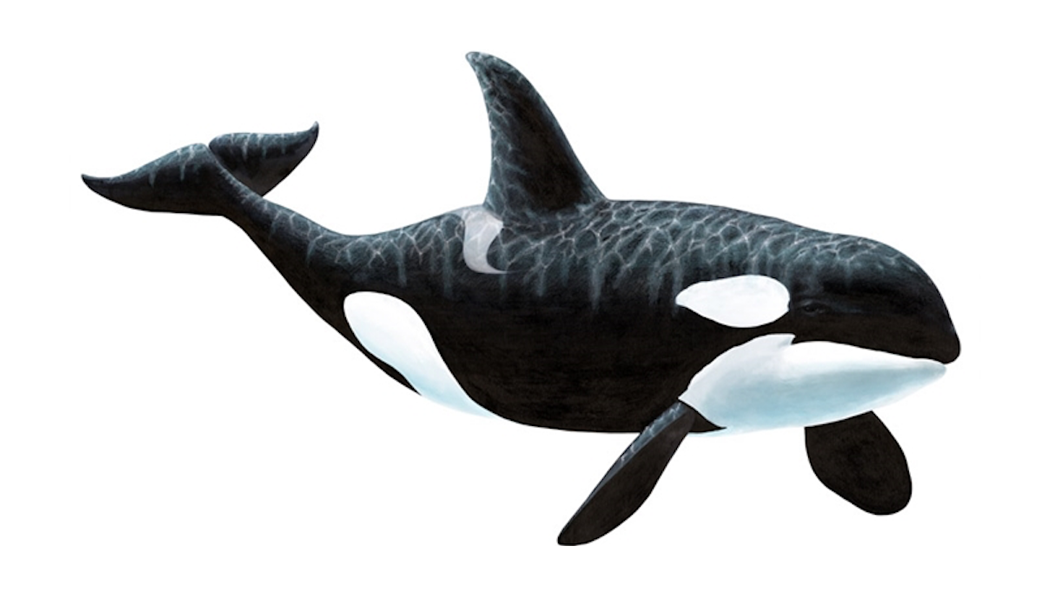
\includegraphics[width=0.9\textwidth]{whale}} 
        \caption{\newline Whale Image}
    \end{minipage}\hfill
    \begin{minipage}{0.33\textwidth}
        \centering
       \fbox{ \includegraphics[width=0.9\textwidth]{whale-1000-initial-before}} 
        \caption{Before}
    \end{minipage}\hfill
    \begin{minipage}{0.33\textwidth}
        \centering
        \fbox{\includegraphics[width=0.9\textwidth]{whale-1000-initial-after}} 
        \caption{After}
    \end{minipage}
\end{figure}

\hfill

\centerline{
\textbf{Code Changes in \textit{hedcut.cpp}:}
}

\begin{figure}[!htb]  
\resizebox{\textwidth}{!}{%
\begin{minipage}{0.48\textwidth}
\centering
\fbox{ \includegraphics[height=5.2cm]{improve1_before}}
\caption{Before}
\end{minipage}

\begin{minipage}{0.48\textwidth}
\centering
\fbox{ \includegraphics[height=5.2cm]{improve1_after}}
\caption{After}
\end{minipage}}
\end{figure}

\newpage

\subsection{Improvement 2: Disk Radius more Dynamic}

As mentioned above the diameter of the disks in the Hedcuter method were extremely small and I had to manually increase the radius as an argument in order to even see the disks clearly. Even if I increased the radius enough manually, all the points even the insignificant ones are increased in radius. 

I modified the code by making the disk radius more dynamic through the size of the voronoi cell and the average color of the voronoi cell. The bigger and the more black the voronoi cell is then the bigger the radius of the disk. This was done by using the 
Voronoi method code as reference. 

For example, Figures 15-17 show stippling of Figure 14 using the Hedcuter method with 1000 disks before my modification and after. Notice in Figure 16 that all the points are increased in size, compared to Figure 15, unlike in Figure 17. More specifically, if you look at the points on my face, in Figure 17 they are smaller compare to Figure 15, which makes the image look better. 

\hfill

\begin{figure}[!htb]
    \centering 
    \begin{minipage}{0.48\textwidth}
        \centering
       \fbox{ 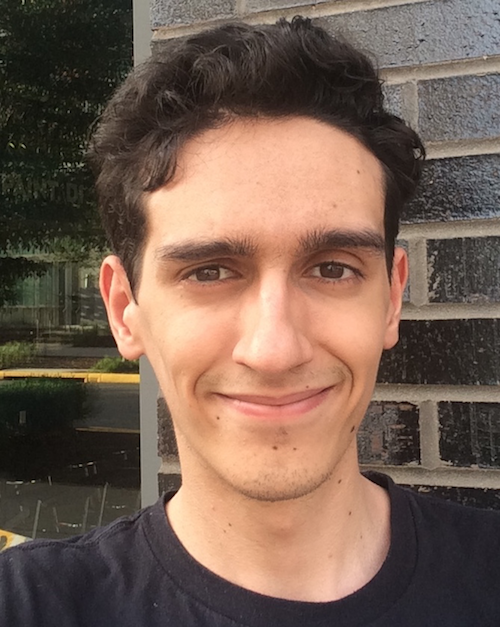
\includegraphics[width=0.6\textwidth]{julian}} 
        \caption{Original Image of Me}
    \end{minipage}\hfill
    \begin{minipage}{0.48\textwidth}
        \centering
       \fbox{ \includegraphics[width=0.6\textwidth]{julian-1000-before-4}} 
        \caption{Before (radius = 4)}
    \end{minipage}
\end{figure}

\begin{figure}[!htb]
    \begin{minipage}{0.48\textwidth}
        \centering
        \fbox{\includegraphics[width=0.6\textwidth]{julian-1000-before-10}} 
        \caption{Before (radius = 10)}
    \end{minipage}\hfill
    \begin{minipage}{0.48\textwidth}
        \centering
        \fbox{\includegraphics[width=0.6\textwidth]{julian-1000-after}} 
        \caption{After}
    \end{minipage}
\end{figure}

\newpage

\centerline{\textbf{Code Changes in \textit{hedcut.cpp} in the \textit{create\_disks} method:}}

\begin{figure}[!htb]  
\resizebox{\textwidth}{!}{%
\begin{minipage}{0.48\textwidth}
\centering
\fbox{ \includegraphics[height=6.2cm]{improve2_hedcut_before}}
\caption{Before}
\end{minipage}

\begin{minipage}{0.48\textwidth}
\centering
\fbox{ \includegraphics[height=6.2cm]{improve2_hedcut_after}}
\caption{After}
\end{minipage}}
\end{figure}

\hfill

\centerline{\textbf{Code Changes in \textit{wcvt.h} in the first \textit{move\_sites} method}}
\centerline{\textbf{(move\_sites(cv::Mat \&  img, VorCell \& cell)):}}

\hfill

\begin{figure}[!htb]
    \centering 
    \fbox{ \includegraphics[width=0.8\textwidth]{improve2_wcvt_move_sites_before}} 
    \caption{Before}
\end{figure}

\begin{figure}[!htb]
    \centering 
    \fbox{ \includegraphics[width=0.8\textwidth]{improve2_wcvt_move_sites_after}} 
    \caption{After}
\end{figure}

\newpage

\centerline{\textbf{Code Changes in \textit{wcvt.h}:}}

\begin{figure}[!htb]  
\resizebox{\textwidth}{!}{%
\begin{minipage}{0.48\textwidth}
\centering
\fbox{ \includegraphics[height=6cm]{improve2_wcvt_before}}
\caption{Before}
\end{minipage}

\begin{minipage}{0.48\textwidth}
\centering
\fbox{ \includegraphics[height=6cm]{improve2_wcvt_after}}
\caption{After}
\end{minipage}}
\end{figure}


\bibliographystyle{plain}
\bibliography{report}

\end{document}


